\documentclass[12pt, oneside]{article} 
\usepackage[left=15mm, right=15mm, top=10mm]{geometry}
\usepackage{graphicx}
\usepackage{url}
\usepackage{multicol}
\usepackage{lipsum}
\usepackage{mwe}
\usepackage{float}

\begin{document}
\title{Techniques d'attaque - stéganographie}
\author{Tristan BILOT, Nora DELFAU, Enzar SALEMI, Madushan THAMBITHURAI\\EPITA}
\date{31 Mai 2021}
\maketitle

\begin{abstract}
Vous êtes Elliot Hackerman, un expert dans le domaine de l’informatique forensique. NotThatEvilCorp, l'un des leaders mondiaux du marché des logiciels, avait besoin de vos services. Apparemment, ils soupçonnent l'un de leurs employés (un développeur Java) de vendre des informations à la concurrence.
Il nous est mis à disposition 3 emails, dont 1 contenant une image et un autre en contenant 2 (voir Fig. 1).
L'objectif va être de découvrir des informations cachées dans ces images afin de déduire si oui ou non la personne transmet des secrets au concurrent. 
\begin{multicols}{2}
        \begin{figure*}[ht!]
            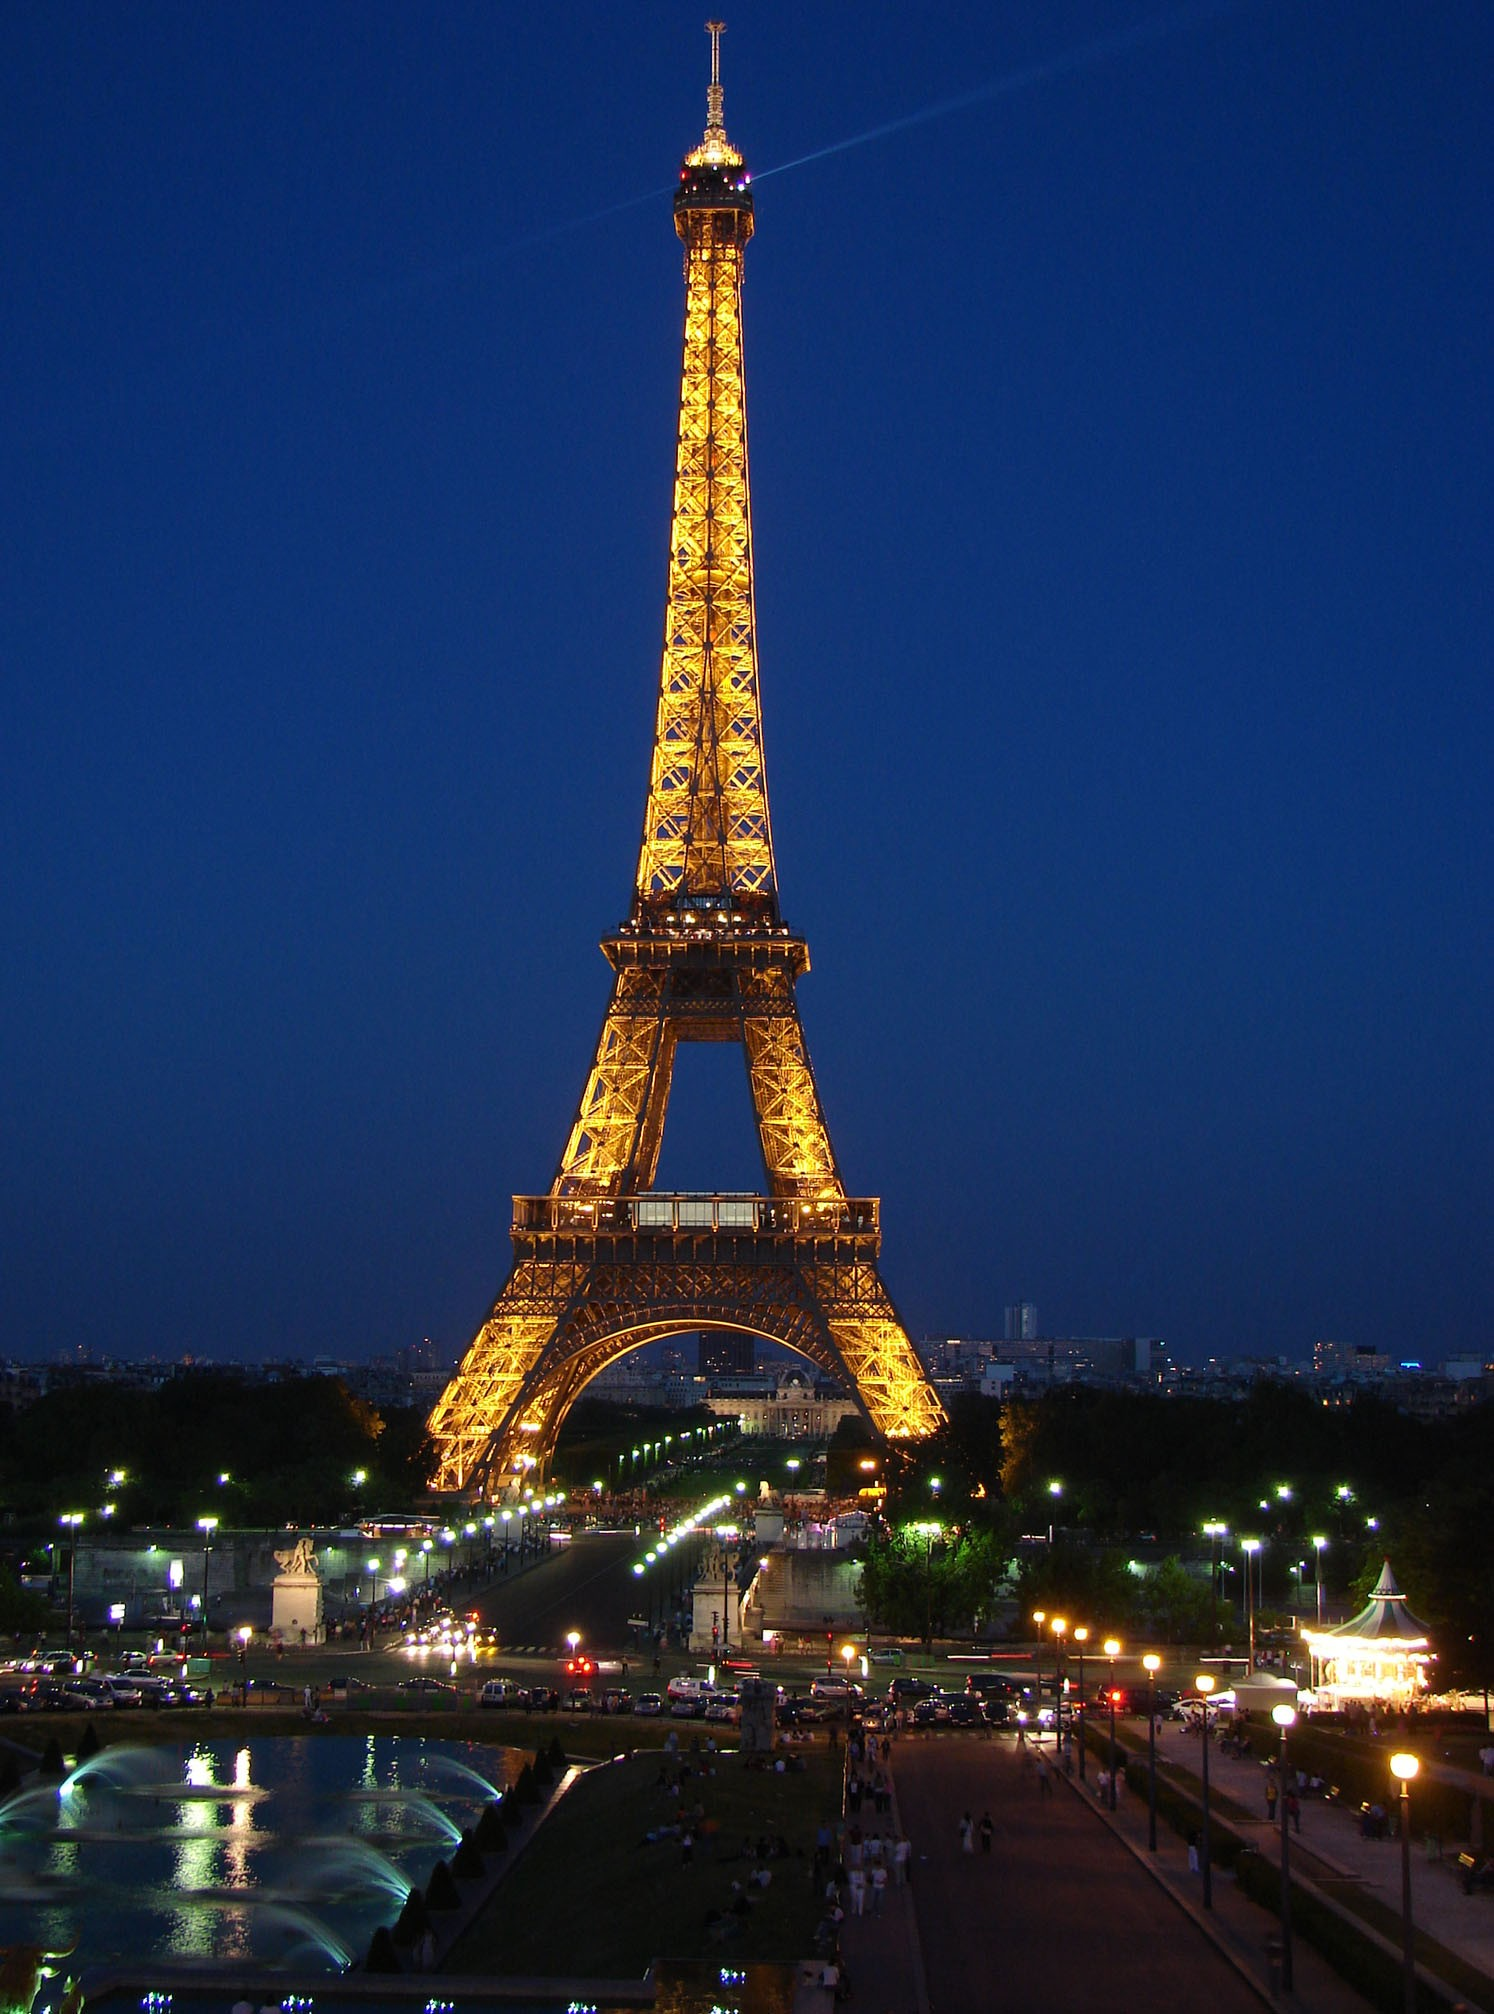
\includegraphics[width=.3\textwidth]{eiffel-img}\hfill
            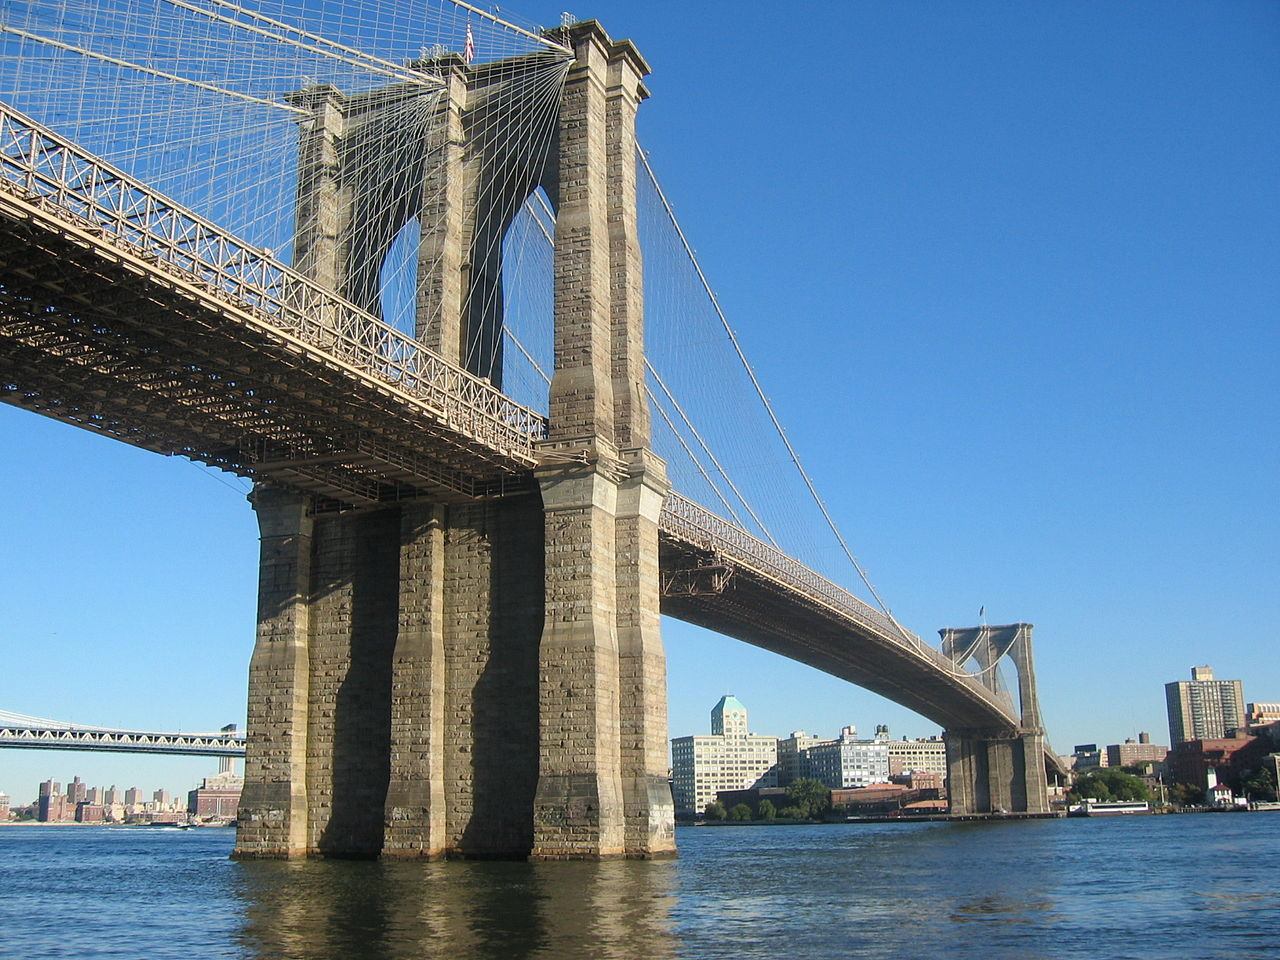
\includegraphics[width=.3\textwidth]{brooklyn-img}\hfill
            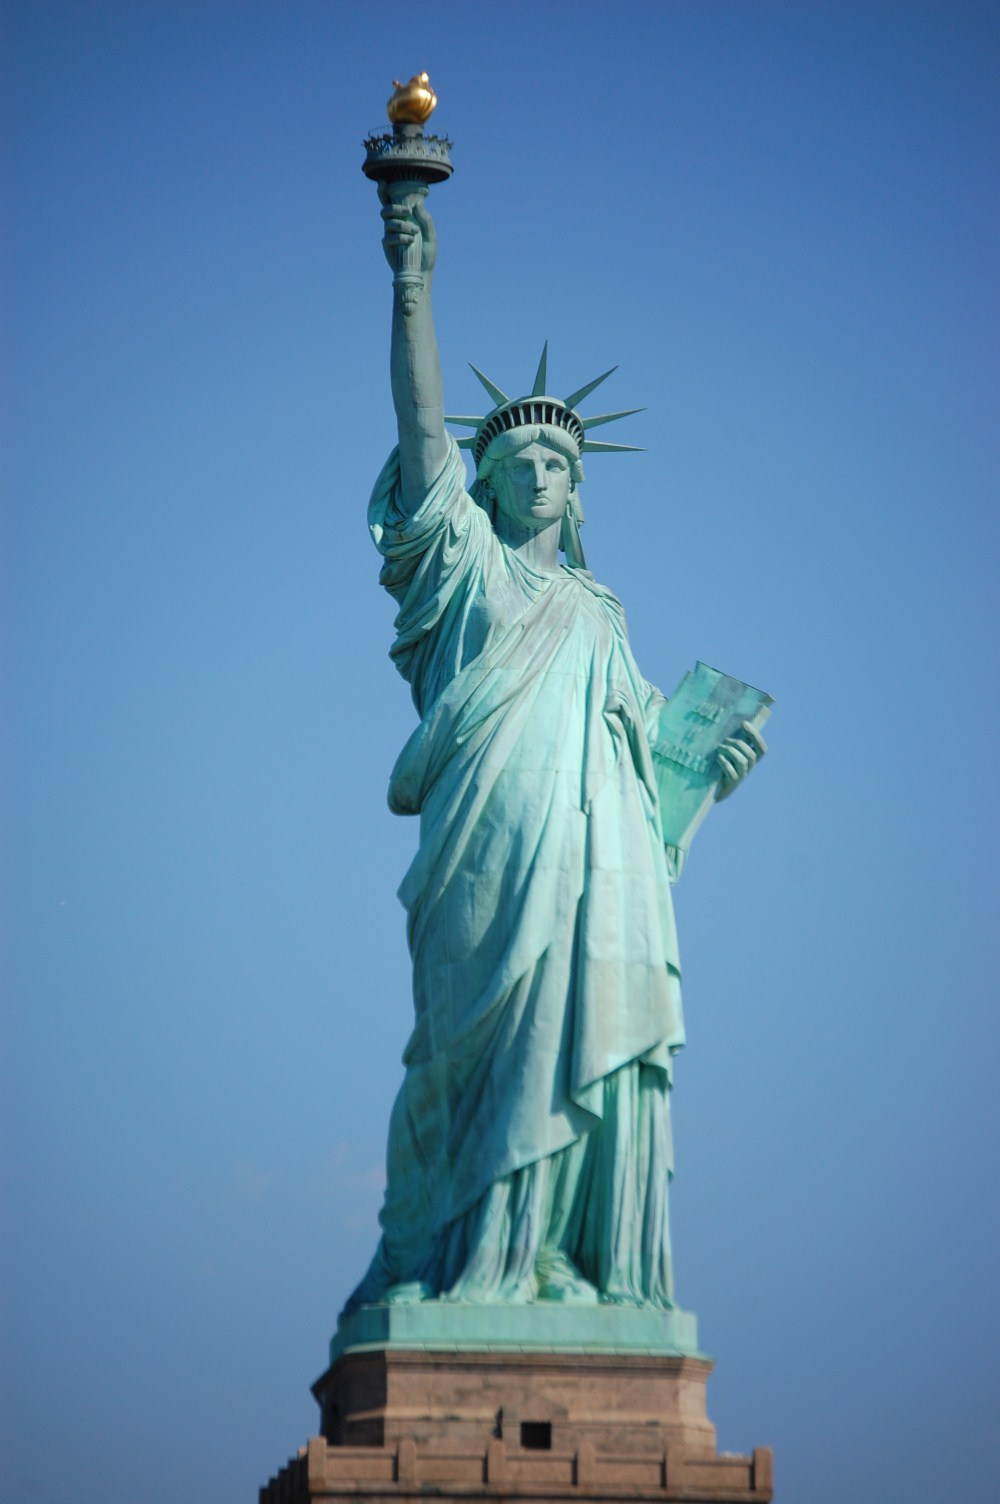
\includegraphics[width=.3\textwidth]{statue-img}
            \caption{Les 3 images à analyser}
        \end{figure*}
    \end{multicols}
\end{abstract}


\section{Notes}
\subsection{Outils fréquemment utilisés}
Elpscrk est un outil de social engineering qui à partir du profil d'une personne, va générer un dictionnaire de mots de passe potentiellement utilisés par une personne cible. 
Hydra est un des outils les plus utilisés et complet pour effectuer des attaques par bruteforce. 
D'autres outils existents comme Brutus, Cain et Abel ou John the Ripper.

\subsection{Rainbow tables}
Dans /etc/shadow, nous trouvons les hashs des mots de passe système. Grâce aux rainbow tables, on peut parvenir à trouver le hash correspondant au mot de passe en utilisant des dictionnaires de hash. 
Les rainbow tables permettent une recherche plus rapide dans ces dictionnaires très longs à parcourir. 
Quand on cible un système, on fait en sorte de connaître à l'avance la méthode de hashage pour avoir le dictionnaire de hashs qui utilise les hashs correspondants à la méthode. 
Stegseek permet de faire de la recherche sur les mots de passe utilisés pour la stéganographie. 

\subsection{Diffie-Hellman}
L'algorithme Diffie-Hellman est utilisé lors de la génération de clés secrètes afin d'établir une connexion sécurisée entre 2 machines. C'est grâce à cela qu'il est possible à Alice et Bob de communiquer de façon sécurisée grâce à leur clé privée sans qu'une troisième personne ne puisse intercepter les messages. On l'utilise notamment lors de l’ouverture d’une connexion à un site sécurisé via le protocole SSL/TLS. De plus, il est omniprésent sur Internet et sur nos smartphones, ce qui en fait un algorithme important à connaître. 

\section{Attaque par dictionnaire sur images}
Dans le cas d'informations cachées dans des images par mot de passe, il peut être intéressant d'utiliser une attaque bruteforce (recherche exhaustive) ou une attaque par dictionnaire (utiliser des mots de passe souvent utilisés afin de maximiser nos chances de trouver le bon mot de passe, souvent créé par un humain et utilisant des inspirations de la vie courante).
Une méthode pourrait être de créer un dictionnaire contenant tous les mots du mail puis d'utiliser ce dictionnaire afin d'essayer d'attaquer l'image grâce à l'outil stegseek. 
Dans un premier temps, construisons donc un dictionnaire contenant l'ensemble des mots contenus dans l'email. 
\begin{figure}[ht]
\centering
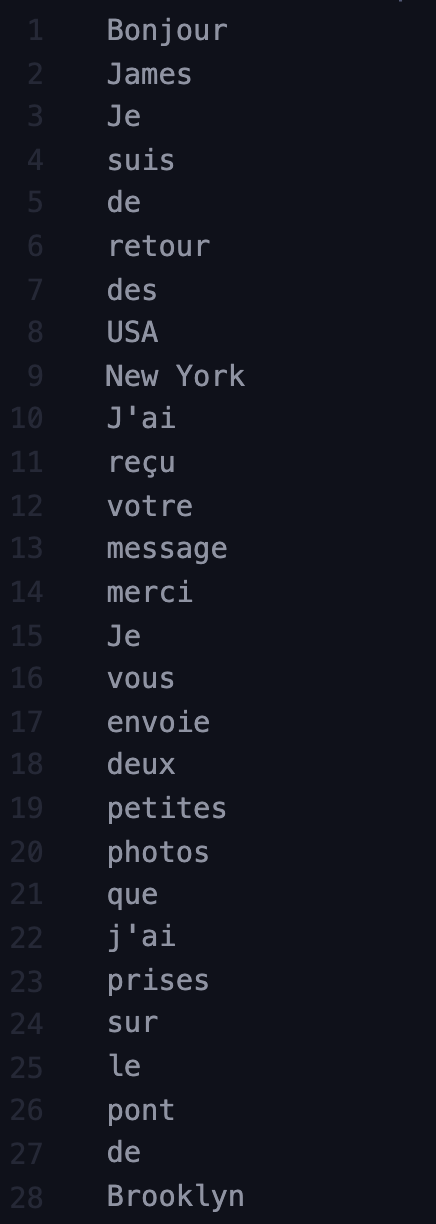
\includegraphics[scale=0.3]{dict}
\caption{Dictionnaire contenant la liste des mots du 1er email}
\end{figure}
A présent, utilisons l'outil stegseek afin d'utiliser un dictionnaire de mots de passe contre une image (Fig. 3). Pour utiliser l'outil stegseek sur MacOS, il est possible d'utiliser docker, sinon il est possible de l'installer directement sur Linux. 
\begin{figure}[ht]
\centering
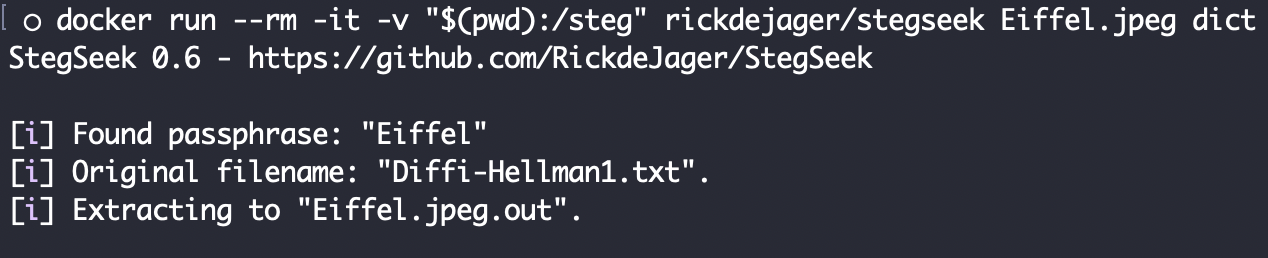
\includegraphics[scale=0.4]{eiffel}
\caption{StegSeek utilisé sur l'image "Tour Eiffel"}
\end{figure}
L'outil retourne bien qu'un mot de passe parmi le dictionnaire a été découvert, dans le cas de l'image de la Tour Eiffel il s'agit du mot de passe "Eiffel". 
De la même façon, nous pouvons trouver les 2 mots de passes des deux autres images: "Brooklyn" (Fig. 4) et "Statue".
\begin{figure}[ht]
\centering
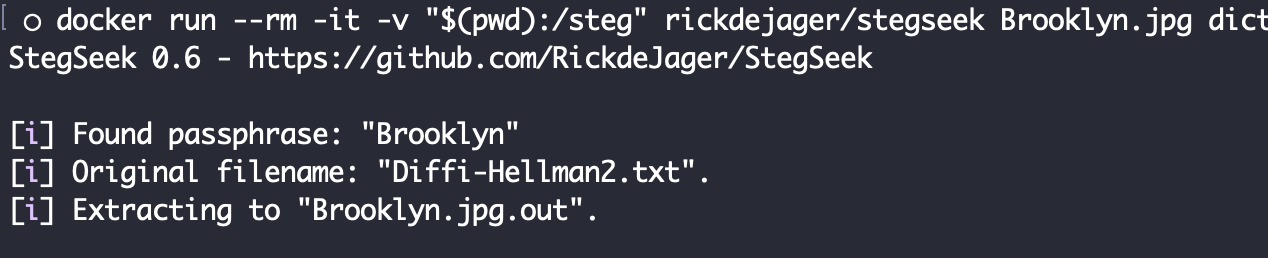
\includegraphics[scale=0.4]{brooklyn}
\caption{StegSeek utilisé sur l'image "Brooklyn"}
\end{figure}

\section{Exfiltration des clés de chiffrement}
Maintenant que nous avons le mot de passe associé à chaque image, nous pouvons poursuivre l'analyse avec l'outil steghide, qui va nous permettre de récupérer les différentes clés utilisées pour le chiffrement des images (Fig. 5). 

\begin{figure}[ht]
\centering
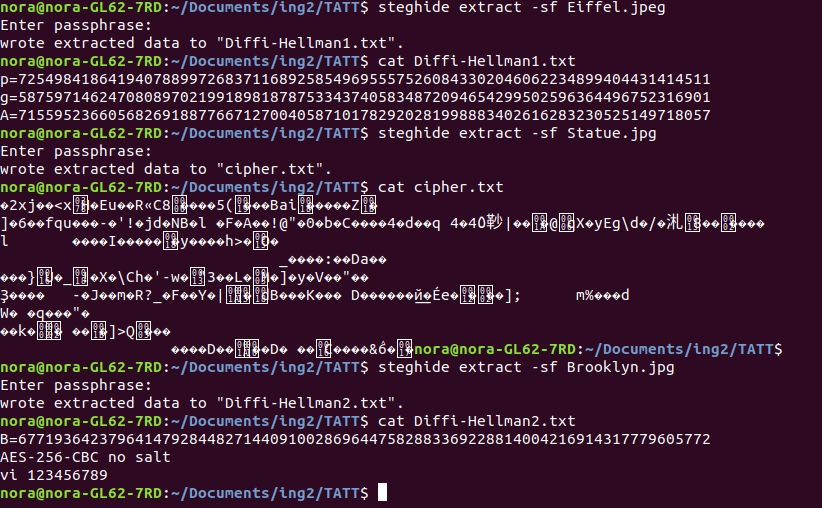
\includegraphics[scale=0.4]{steghide}
\caption{StegHide permettant de récupérer les clés de chiffrement}
\end{figure}

Après utilisation de l'outil, plusieurs fichiers sont générés: 1 fichier cipher.txt contenant le message chiffré en aes-256-cbc et 2 fichiers Diffie-Hellman qui contiennent les clés utilisées pour l'échange de clé lors du chiffrement. Grâce à ces différentes informations, nous sommes presque capable de déchiffrer le message car nous savons que l'algorithme utilisé pour la génération des clés est Diffie-Hellman, et nous avons la plupart des clés. Il ne nous manque plus que la clé privée b afin d'appliquer le déchiffrement. Or, nous savons que la personne à l'origine de ces images est un développeur Java qui a certainement utilisé une génération pseudo-aléatoire pour l'obtention de la clé b. Cette génération aléatoire utilise le timestamp actuel de la machine donc nous pouvons essayer par bruteforce tous les timestamps possibles dans l'intervalle de temps ou la génération de l'image est la plus probable (entre les dates d'envoi des deux emails). Ce qui nous invite à créer un algorithme Java utilisant de la même façon une génération de nombre aléatoire afin de compléter l'équation: 
\[ B = G^b mod P \]
L'algorithme consiste à essayer de résoudre l'équation pour toutes les millisecondes entre l'envoi des 2 messages (Fig. 6). 
Avec cette première méthode, nous nous rendons compte qu'il y a ~2 milliards de millisecondes entre les deux dates, ce qui mettrait un temps conséquent à résoudre. Nous avons donc pensé à regarder la dates de création des images afin de réduire fortement cet intervalle de temps. Grâce à cette amélioration de l'algorithme, nous avons réussi à trouver la clé manquante en seulement quelques secondes.

\begin{figure}[ht]
\centering
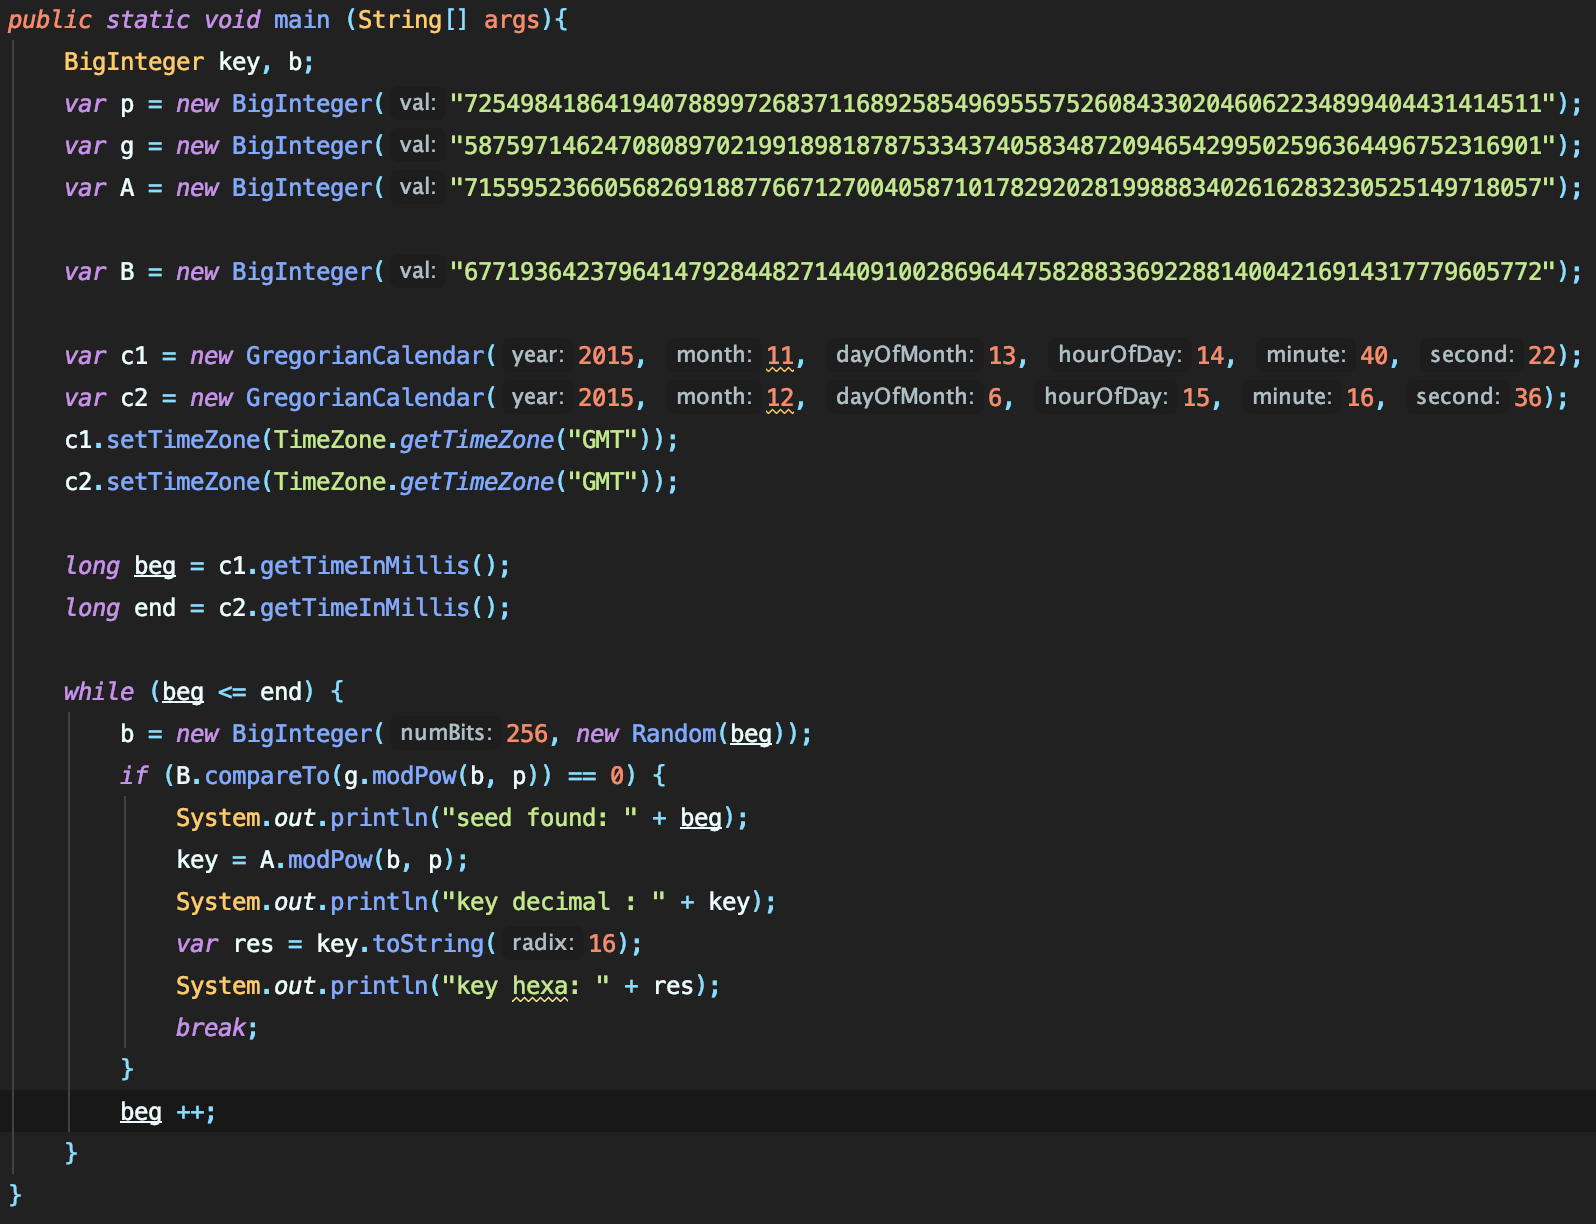
\includegraphics[scale=0.5]{code}
\caption{Algorithme de brutforce de la seed}
\end{figure}

Résultats de l'algorithme: 
\begin{itemize}
  \item random seed: \(1450018437892\)
  \item decimal \(b\) key: \(30899383377856444262432941452181130060109265952665886885841266221802454368037\)
  \item hexa \(b\) key: \(44506e64c6a3de6416c6c3ce567a418371dbbebdc917fc5df61201770365bf25\)
\end{itemize}

\section{Déchiffrement du message}
Il est désormais possible de déchiffrer le message cipher.txt. Pour cela nous utiliserons openssl avec les options -d pour déchiffrer, -aes-256-cbc -nosalt car c'est le mode de chiffrement utilisé initialement, ainsi que l'option -iv définissant le vecteur d'initialisation à utiliser. Pour rappel, dans un mode de chiffrement cbc, le vecteur d'initialisation va servir de source aléatoire pour le 1er bloc à chiffrer, qui lui-même sera utilisé pour le chiffrement des blocs suivants via des XOR par exemple. C'est grâce à cela que l'algorithme peut retourner à chaque chiffrement un résultat différent, et donc être beaucoup plus robuste et fiable. A noter qu'avant d'utiliser la clé b directement avec l'option -K d'openssl, il est nécessaire de convertir la clé en base hexadécimal, ce qui est effectué directement par l'algorithme Java. 
\begin{figure}[ht]
\centering
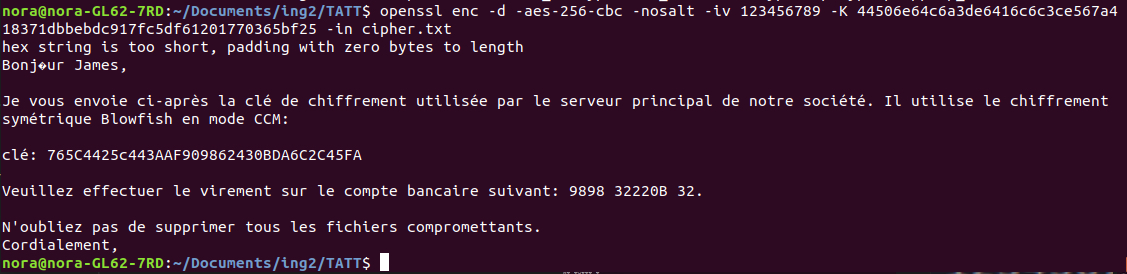
\includegraphics[scale=0.4]{answer}
\caption{Déchiffrement final du message}
\end{figure}
Enfin, nous arrivons à déchiffrer le message secret initialement caché dans l'image, grâce aux clés.

\end{document} 

